
% LaTeX2e document class file for submissions to sigkdd explorations.
% It is an example which *does* use the .bib file (from which the .bbl file
% is produced).
% REMEMBER HOWEVER: After having produced the .bbl file,
% and prior to final submission,
% you need to 'insert'  your .bbl file into your source .tex file so as to provide
% ONE 'self-contained' source file.
%
% Questions regarding SIGS should be sent to
% Adrienne Griscti ---> griscti@acm.org
%
% Questions/suggestions regarding the guidelines, .tex and .cls files, etc. to
% Gerald Murray ---> murray@acm.org
%

\documentclass{sigkddExp}
%\usepackage{geometry}
%\usepackage[a4paper,bindingoffset=0in,%
% left=0.5in,right=0.3in,top=0.5in,bottom=0.3in,%
%             footskip=0in,hoffset=-0.5in, voffset=-0.4in]{geometry}
\usepackage[authoryear,round,longnamesfirst]{natbib}
\usepackage{url,amsmath,amsfonts,amssymb}
\usepackage{caption}
\usepackage{subcaption}
\usepackage{algorithm}
\usepackage[noend]{algpseudocode}
\usepackage{graphicx}
\usepackage{listings}
\usepackage[T1]{fontenc}
\usepackage{enumerate}   
\usepackage{color}
\usepackage{relsize}
\usepackage{inputenc}
\usepackage{multirow}


\newtheorem{definition}{Definition}
\newtheorem{remark}{Remark}
\newtheorem{properties}{Properties}
\newtheorem{example}{Example}
\newtheorem{theorem}{Theorem}
\newtheorem{lemma}[theorem]{Lemma}
\newtheorem{corollary}[theorem]{Corollary}
\newtheorem{proposition}[theorem]{Proposition}
\newtheorem{claim}[theorem]{Claim}
\newtheorem{observation}{Observation}

%\def \endprf{\hfill {\vrule height6pt width6pt depth0pt}\medskip}
%\newenvironment{proof}{\noindent {\bf Proof} }{\endprf\par}

\newcommand{\R}{{\mathbb R}}
\newcommand{\Z}{{\mathbb Z}}
\newcommand{\Q}{{\mathbb Q}}
\newcommand{\C}{{\mathbb C}}
\newcommand{\N}{{\mathbb N}}
\newcommand{\B}{{\mathbb B}}
\newcommand{\bz}{{\mathbf z}}
\newcommand{\bh}{{\mathbf h}}
\newcommand{\bff}{{\mathbf f}}
\newcommand{\bdelta}{{\mathbf \delta}}
\newcommand{\bsigma}{{\mathbf \sigma}}
\newcommand{\bmu}{{\mathbf \mu}}

\newcommand{\M}{{\mathcal M}}
\newcommand{\F}{{\mathcal F}}
\newcommand{\E}{{\mathbb E}}
\newcommand{\A}{\mathcal{A}}
\newcommand{\I}{\mathbb{I}}
\newcommand{\U}{\mathcal{U}}
\newcommand{\V}{\mathcal{V}}


\newcommand{\Prob}{\mathbb{P}}
\newcommand{\di}{{i\mkern1mu}}


\newcommand{\Var}{\textit{var}}




 \setlength{\oddsidemargin}{0pt}
 \setlength{\evensidemargin}{0pt}
 \setlength{\textwidth}{6.7in}
 \setlength{\topmargin}{0in}
 \setlength{\textheight}{8.5in}

 
\begin{document}
%
% --- Author Metadata here ---
% -- Can be completely blank or contain 'commented' information like this...
%\conferenceinfo{WOODSTOCK}{'97 El Paso, Texas USA} % If you happen to know the conference location etc.
%\CopyrightYear{2001} % Allows a non-default  copyright year  to be 'entered' - IF NEED BE.
%\crdata{0-12345-67-8/90/01}  % Allows non-default copyright data to be 'entered' - IF NEED BE.
% --- End of author Metadata ---

\title{Bayesian Embedding --- a generic framework for incorporating prior knowledge into graph embedding }
%\subtitle{[Extended Abstract]
% You need the command \numberofauthors to handle the "boxing"
% and alignment of the authors under the title, and to add
% a section for authors number 4 through n.
%
% Up to the first three authors are aligned under the title;
% use the \alignauthor commands below to handle those names
% and affiliations. Add names, affiliations, addresses for
% additional authors as the argument to \additionalauthors;
% these will be set for you without further effort on your
% part as the last section in the body of your article BEFORE
% References or any Appendices.

\numberofauthors{6}
%
% You can go ahead and credit authors number 4+ here;
% their names will appear in a section called
% "Additional Authors" just before the Appendices
% (if there are any) or Bibliography (if there
% aren't)

% Put no more than the first THREE authors in the \author command
%%You are free to format the authors in alternate ways if you have more 
%%than three authors.

\author{
%
% The command \alignauthor (no curly braces needed) should
% precede each author name, affiliation/snail-mail address and
% e-mail address. Additionally, tag each line of
% affiliation/address with \affaddr, and tag the
%% e-mail address with \email.
\alignauthor Yuting Ye \\
       \affaddr{~}\\
       \affaddr{~}\\
       \affaddr{~}\\
       \email{~}
\alignauthor Xuwu Wang\\
       \affaddr{~}\\
       \affaddr{~}\\
       \affaddr{~}\\
       \email{~}
% \alignauthor Lars Th{\o}rv\"{a}ld\titlenote{This author is the
% one who did all the really hard work.}\\
%        \affaddr{The Th{\o}rv\"{a}ld Group}\\
%        \affaddr{1 Th{\o}rv\"{a}ld Circle}\\
%        \affaddr{Hekla, Iceland}\\
%        \email{larst@affiliation.org}
}     
%\additionalauthors{Additional authors: John Smith (The Th{\o}rvald Group,
%email: {\texttt{jsmith@affiliation.org}}) and Julius P.~Kumquat
%(The Kumquat Consortium, email: {\texttt{jpkumquat@consortium.net}}).}

    
%\date{28 December 2018}
\maketitle
\begin{abstract}
This paper provides a Bayesian framework, called BEM (Bayes EMbedding) that bridges the knowledge graph and entity-specific information. This framework is highly flexible in that it can take as input either the raw data or pre-trained embeddings. On the one hand, BEM can mutually correct the embeddings from two sides, one from the knowledge graph and the other one from the entity information. The corrected embeddings are enriched with the information from the other side. On the other hand, BEM holds the promise of making an end-to-end embedding network that uses the knowledge graph to guide the downstream embedding learning. Extensive experiments have been done to display the efficacy of BEM.
\end{abstract}

\section{Introduction}
\section{Methods}

\subsection{Notation}

\subsection{Models of BEM}
The motivation of BEM originates from the cognitive science. Human beings's understanding process works in two systems: (System I) unconsciously retrieves pieces of knowledge associated with the given task; (System II) subjectively use analytic reasoning to analyze or ponder the received information. In spirit, the triplets in the knowledge graph function and distribute similarly to the knowledge used in System I: they provide association rather than causlity; they are scattered around rather than organized. Therefore, we are motivated to design a model that mimics System II. The triplets in the knowledge graph are regarded as the base knowledge that will be further processed to solve a specific task. In other words, the embedding from the knowledge graph should be corrected in terms of the task to tackle.

We first start with the simplest case where each entity has two embeddings, one from the knowledge graph and the other given by a specific task. For an entity $e$, we suppose that the task-specific embedding $\bz_{e}$ is generated from a distribution determined by the knowledge graph embedding  $\bh_{e}$ and a correction term with $\bdelta_e$ respect to the task, that is,
\begin{equation}
  \bz_{e} \approx \bff(\bh_e + \bdelta_e),
  \label{eq:connection_z_h_1st}
\end{equation}
where $\bff$ is a non-linear function that projects $\bh_e + \bdelta_e$ as $\bz_e$. However, both $\bz_e$ and $\bh_e$ are distributed on the sphere. The set of all $\bz_{e}'s$ (or $\bh_{e}'s$) is the same for the downstream goal such as classification or prediction, up to a variety of operations including rotation and reflection. A sufficiently complicated non-linear function $\bff$ is required to express such operation. However, the number of parameters are obviously larger than the sample size, since each entity needs a correction term. Learning $\bdelta_e$'s and $\bff$ seems infeasible. On the other hand, we note that the learnings of both the knowledge graph embeddings and the task-specific embeddings are highly dependent on the interaction between entities. Decoupling the second-order information between entities as \eqref{eq:connection_z_h_1st} might lead to an intolerable loss regarding the goal for a good embedding. Considering the interaction not only retains the loss of key information, but also increases the sample sizes (there are $N_e^2$ pairs of entities). With these considerations, we formulate a generation model from $\bh_e$ to $\bz_e$:
\begin{itemize}
\item [1.] For each entity $e$:
  \begin{itemize}
	\item sample its correction variable $\bdelta_e \sim N(\bold 0, \lambda_1 \cdot s_h^2)$, where $\lambda_1$ is a tuning parameter and $s_h^2$ is estimated by $\bold h_e$.
	\item sample its assoiated uncertainty variable $\bsigma_{e_j}^2 \sim \text{log~Normal}(\ell_{\mu_e}, \lambda_2\cdot \ell_{\sigma^2_e})$, where $j = 1, \ldots, d_2$. Here, $\ell_{\mu_e}$, $\ell_{\sigma^2_e}$ can be estimated by $\bold z_e$'s, and $\lambda_2$ is a tuning parameter.
      \end{itemize}
    \item [2.] For each pair of entities, $e_1$, $e_2$, sample
      \begin{equation}
        \bold z_{e_1} - \bold z_{e_2} \sim  N\left ( \bff_{\phi}(\bh_{e_1} +  \bdelta_{e_1}) - \bff_{\phi}(\bh_{e_2} + \bdelta_{e_2}), \text{diag}(\bsigma_{e_1}^2 + \bsigma_{e_2}^2) \right),
        \label{eq:connection_z_h_2nd}
        \end{equation}
where $\bff_{\phi}$ is a neural network with parameter $\phi$. 
\end{itemize}
The model is depicted in Figure \ref{fig:generation_model} as well. Our goal is to seek the best parameter $\phi$ and the posteriors of $\bdelta_e$'s, $\bsigma_{e_j}$'s in \eqref{eq:connection_z_h_2nd}, given all the $\bh_e$'s and $\bz_e$'s. Suppose the fitted network paramter is $\hat{\phi}$ and the posterior mean of $\bdelta_e$ is $\hat{\bmu}_{e}$, we use $\bh_e +\hat{\bmu}_{e}$ as the corrected embedding for the knowledge graph, and $\bff_{\hat{\phi}}(\bh_e +\hat{\bmu}_{e})$ as the corrected embedding for the specific task.

\begin{figure}[h]
  \centering
  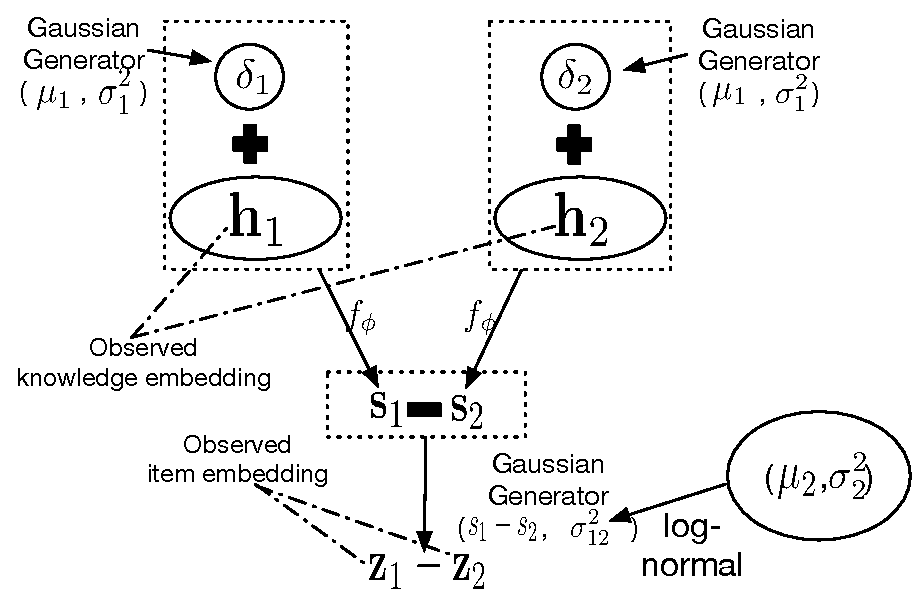
\includegraphics[width=0.5\textwidth]{./fig/generation.pdf}
  \caption{The BEM model.}
  \label{fig:generation_model}
\end{figure}
\subsection{Algorithm of BEM}


\section{Experiments}

\subsection{Data description}
We mainly use two datasets for evaluation. One dataset is a subset of E-commerce data from Alibaba on November 28th for the mother\&baby scenario, termed as \textit{Alibaba-MB}. In this dataset, we have $377,183$ items, each of which has $22$ continuous attributes and $10$ discrete attributes (details of the attributes are deferred to the appendix). All these attributes appear as the head entity in $5,565,558$ triplets. There are $1,931$ relations ($2,000$ properties for ``HasProperty'', ``IsInstanceOf'', ``BelongToScenario'') and tail entities ($430$ categories, $1,511,000$ values, $111,000$ concepts). Another dataset is the public dataset \textit{FBK15}. It has $14,904$ entities appearing as both the heads and tails in $579,655$ triplets. For each entity, we find an associated short paragraph in the database \textit{freebase} that describes the entity.


\subsection{Embedding correction}
We first investigate the performance of BEM for embedding correction. For the dataset \textit{Ali-MB}, the item attributes, along with item graph obtained by user behaviour, are used to get the item embeddings by \textit{GraphSAGE}. For the dataset \textit{FBK15}, the entity-specific description paragraphs are fed into \textit{doc2vec} for embeddings. As with the knowledge graph, \textit{TransE} (we utilize the implementation from the OpenKE library) is used to obtain the embeddings using the triplets. We call the embeddings from item attribute as ``embedding(item)'', the embeddings from the description paragraphs as ``embedding(desc)'',  and those from knowledge graph as ``embedding(kg)'' respectively. Multiple tasks are studied to compare the embeddings before and after the correction by BEM.

\subsubsection{Item Prediction for \textit{Alibaba-MB}}\label{sec:item_pred_ali_mb}
There are two classification tasks, that is, to predict item categories of level 1 (L1) and level 2 (L2). We have $83$ L1 categories and $580$ L2 categories. The evluation measurement for this task is $\text{classification accuracy}:= \#\{\text{correctly classified items}\}/\#\{\text{total items}\}$. In addition, we execute two regression tasks, that is, to predict item prices and item popularities. We use the squared $\ell_2$ norm for evaluation. We note that the category information is used in the training of item embedding and knowledge graph embedding, while the item price and popularity are only used in the training of item embedding. We use a one-hidden-layer MLP with $32$ hidden nodes for classification or regression. 

Table \ref{tbl:item_pred_ali_mb} displays the results of the four tasks for item embeddings and kg embeddings before and after correction by BEM respectively. The extremely high accuracy of the two classification tasks results from the leaky information ---  the features partially include the predictors. Nevertheless, the knowledge graph and item attributes see different degrees of leak. It seems that the original embedding(item) is better informed of the categories than the original embedding(kg). After correction, the embedding(kg) always benefits from getting information from the other side in terms of classification accuracy, while the result of the embedding(item) gets worse for the level-2 category. It verifies the fundamental motivation of BEM that it merges two sides of embeddings. As with the two regression tasks, we observe similar results as the classification tasks. The item attributes include the price level but the knowledge graph does not, thus the original embedding(item) has a lower loss than the corrected one. The corrected embedding(kg) is obviously benefitted from learning the embedding(item). As for the task of predicting the item popularity, the predictors concentrate on low values but there are quite a few outliers. Therefore, the results display a high variance that masks the same trend as the task of predicting the price.



\begin{table}[h]
  \caption{Classification/Regression results for BEM on the \textit{Alibaba-MB} dataset. Predictors category(L1/L2) correspond to using level1/level2 category for classification, while predictors price level/popularity correspond to using the item price or the item popularity for regression.}
  \label{tbl:item_pred_ali_mb}
  \centering
\begin{tabular}{l|l|l|l|l}
\hline
Predictor      & \multicolumn{2}{l|}{embedding (item)} & \multicolumn{2}{l}{embedding (kg)} \\ \hline
              & original          & corrected         & original         & corrected        \\ \hline
category(L1) & 99.24\%           & 99.31\%           & 95.87\%          & 98.99\%          \\ 
category(L2) & 96.93\%           & 94.06\%           & 90.89\%          & 96.86\%          \\ 
price level   & 0.5392            & 0.6935            & 0.9309           & 0.6644           \\ 
popoularity   & 1852              & 1962              & 2008             & 1977             \\ \hline
\end{tabular}
\end{table}

\subsubsection{Link Prediction \& Triplet Classification for \textit{FBK15}}
Two tasks are done to study the performance of BEM on the \textit{FBK15} dataset, i.e., link prediction (LP) and triplet classification (TC). Both the two tasks are executed using the default APIs from the OpenKE library, given the embeddings from the knowledge graph.

The results for the two task with different parameters are presented in Table \ref{tbl:tune_par_fbk15}. The \textit{default} setting only uses the \textit{TransE} method without the BEM correction and with parameters $\#\text{epochs} = 500$, $\# \text{batches} = 100$, $\text{learning~rate} = 0.001$, $\text{margin} = 1.0$, $\text{embedding~dimension} = 100$, and etc.. The \textit{noisy} setting only trains the relation embeddings while leaving the entity embeddings as initialized. The two \textit{Tune-TransE} settings have exactly the same parameters as the \textit{default} setting except for the ones they specify. As for the six settings in \textit{Tune-BEM}, they utilize the BEM method to incorporate the information from the description paragraphs into the embedding(kg). The setting with $\text{learning rate} = 0.001$ is exactly the same parameters for \textit{TransE} as the \textit{default} one. Its parameters for BEM are $\lambda_1 = 1.0$, $\lambda_2 = 1.0$, $\# \text{epochs} = 20$, $\# \text{batches} = 500$, $\text{learning~rate} = 0.001$. Other settings differs from the setting with $\text{learning rate} = 0.001$ only in the parameter they specify.

The results of corrected embedding(kg) are inferior to those of the original embeddings in the task of link prediction and triplet classification. This results from the fact that the description paragraphs do not contain sufficient information about knowledge graph triplets to benefit the other side. A direct implication is that the results of the corrected embedding(kg) get worse as more information from the description paragraphs is incorporated into it. On the other hand, we still get valuable insight by comparing the results between distinct parameters. $\lambda_1$ and $\lambda_2$ play the role of coefficients that adjust the trade-off between the reconstruction term and the penality term (KL divergence). Small $\lambda_1$ forces the corrected embedding(kg) to get close to the original one while small $\lambda_2$ forces any pair of the corrected embeddings(desc) to distribute as far as the original pair. 


\begin{table*}[h]
  \caption{Link prediction (LP)/Triplet classification (TC) results for BEM on the \textit{FBK15} dataset. The result with one tuning parameter (except for tuning BEM) only differs in this parameter from the default. The result with one tuning parameter (for tuning BEM) only differs in this parameter from the setting of $\text{learning rate = } 0.001$.}
  \label{tbl:tune_par_fbk15}
  \centering
\begin{tabular}{l|l|l|l|l|l|l|l|l|l|l|l}
\hline
  task        &metrics  & default & noisy  & \multicolumn{2}{c|}{Tune-TransE} &  \multicolumn{6}{c}{Tune-BEM} \\ \hline
         &  &  & & (batch, epoch) & dim & \multicolumn{2}{c|}{learning rate} & \multicolumn{2}{c|}{$\lambda_1$} & \multicolumn{2}{c}{$\lambda_2$} \\ \hline
            & & & & ($800, 1000$) & $50$ & $0.001$ & $0.005$ & $0.1$ & $2$ & $0.1$ & $2$ \\ \hline
  \multirow{4}{*}{LP} & MR & $63$ & $5693$ & $69$ & $66$ & $82$ & $69$ & $65$ & $93$ & $79$ & $73$  \\
             & hit@10& $71.83\%$ & $8.39\%$ & $76.11\%$ & $62.97\%$ & $60.26\%$ & $63.55\%$ & $67.24\%$ & $55.25\%$ & $59.00\%$ & $62.34\%$ \\
             & hit@5 & $54.41\%$ & $7.43\%$ & $59.08\%$ & $45.19\%$ & $41.45\%$ & $47.59\%$ & $48.84\%$ & $37.25\%$ & $40.61\%$ & $43.62\%$ \\
             & hit@1 & $32.60\%$ & $6.58\%$ & $35.56\%$ & $26.88\%$ & $21.49\%$ & $25.86\%$ & $26.65\%$ & $19.76\%$ & $21.59\%$ & $23.61\%$ \\\hline
  TR & accuracy & $85.99\%$ & $52.67\%$ & $87.48\%$ & $85.28\%$ & $82.65\%$ & $84.01\%$ & $85.50\%$ & $80.73\%$ & $82.27\%$ & $83.38\%$ \\\hline
  
\end{tabular}
\end{table*}


\subsubsection{Entity Classification for \textit{FBK15}}
We investigate the performance the corrected embeddings(desc) and embeddings(kg) obtained from the \textit{FBK15} dataset on another task. We note that the relations in this dataset not only contains the true relation between the head entity and the tail entity, but also include the domain and category words potentially associated with the entities. We retrieve the category labels for each entity from all the relations it is connected with in existing triplets. One entity can have multiple labels and we use the one of the highest occurence across all entities. We are aware that such label is not perfectly reliable due to the potentially leaky information during the training of the embedding(kg) and the naive selection of labels. Once the embeddings are obtained, the classification task is done via a one-hidden-layer MLP with $32$ hidden nodes.

Tabel \ref{tbl:entity_class_fbk15} displays the classification accuracy of the corrected embeddings in contrast to the orignal ones. We study the embedding(desc), the embedding(kg) and the embedding obtained by concatenating both of them. The original embedding(kg) can better distinguish the entity category, which implies that the training process sees partial information about the labels. We note that the embeddings by concatnating the original two types of embeddings perform better than single embeddings regardless of whether corrected or not. It is easily understood since the concatenation operation does not lose information from both sides in distinction to BEM. However, BEM obviously benefits the embeddings in that all the corrected ones are superior to the corresponding orignal ones. And the corrected embedding(kg) attains pretty close accuracy as the orinal concatenated embedding. It is not fully clear whether the gap is caused by the more expressive classifier for the concatenated embedding (its input size is double that of the single embedding). In fact, the single embedding and the concatnated embedding are not directly comparable. Still, we see that the BEM implicitly increases the singal-to-ratio even for the concatenated embeddings with respect to the task of classifying entity labels.

\begin{table}[h]
  \caption{Classification results for BEM on the \textit{FBK15} dataset. The abbreviation \textit{desc} refers to embeddings from entity-specific description paragraphs, \text{kg} refers to the embeddings from the knowledge graph, \text{concat} refers to concatenting the desc embeddings nd the kg embeddings.}
  \label{tbl:entity_class_fbk15}
  \centering
\begin{tabular}{l|l|l|l}
\hline
          & \multicolumn{3}{c}{embedding} \\ \hline
          & desc     & kg       & concat   \\ \hline
original  & 62.10    & 68.19    & 72.33    \\ 
corrected & 66.01    & 72.00    & 73.83    \\ \hline
\end{tabular}
\end{table}

\subsection{End-to-end learning by BEM}
 
\section{Discussion}

%
% The following two commands are all you need in the
% initial runs of your .tex file to
% produce the bibliography for the citations in your paper.
\bibliographystyle{abbrv}
\bibliography{Bayes_Em}  % sigproc.bib is the name of the Bibliography in this case
% You must have a proper ".bib" file
%  and remember to run:
% latex bibtex latex latex
% to resolve all references
%
% ACM needs 'a single self-contained file'!
%
%APPENDICES are optional
% SIGKDD: balancing columns messes up the footers: Sunita Sarawagi, Jan 2000.
% \balancecolumns
%\appendix

% That's all folks!
\end{document}
